\section{Research} % (fold)
\label{sec:research}
The research component can be split into two components - the GUI \textbf{visualizer} and the search method \textbf{analysis} component.

\subsection{Visualizer} % (fold)
\label{sub:visualizer}
To be able to both verify the behavior of each search algorithm and to demonstrate to others how each method affects its search tree, a GUI visualizer was developed as a research component. It can be opened via the same CLI application as the assignment component using the \mintinline[bgcolor=codebg]{shell}{./robonav -v} option. This will open the visualizer app - a grid with cells representing states in the search space - black cells are walls, the red cell is the start state, and the green cell is the goal.

\paragraph{Usage} % (fold)
\label{par:usage}
Both the start and end state can be moved by clicking and dragging, while walls can be placed and removed by clicking in empty spaces. The keys \textbf{1 - 6} are used to choose each search algorithm, \textbf{space} clears the current path and \textbf{enter} begins a search. To quit press the \textbf{escape} key.
% paragraph usage (end)

\paragraph{Visuals} % (fold)
\label{par:visuals}
The visualization of each search algorithm is not in real-time but in a time proportional to the amount of operations each one made. The visualizer displays each operation as it happened in order as denoted by the moving orange cell (the current node in the search tree), explored nodes are denoted as light blue which are added as the search tree expands. Finally, once the goal is found, the path taken to reach it is highlighted green.
% paragraph visuals (end)

\begin{figure}[H]
	\centering
	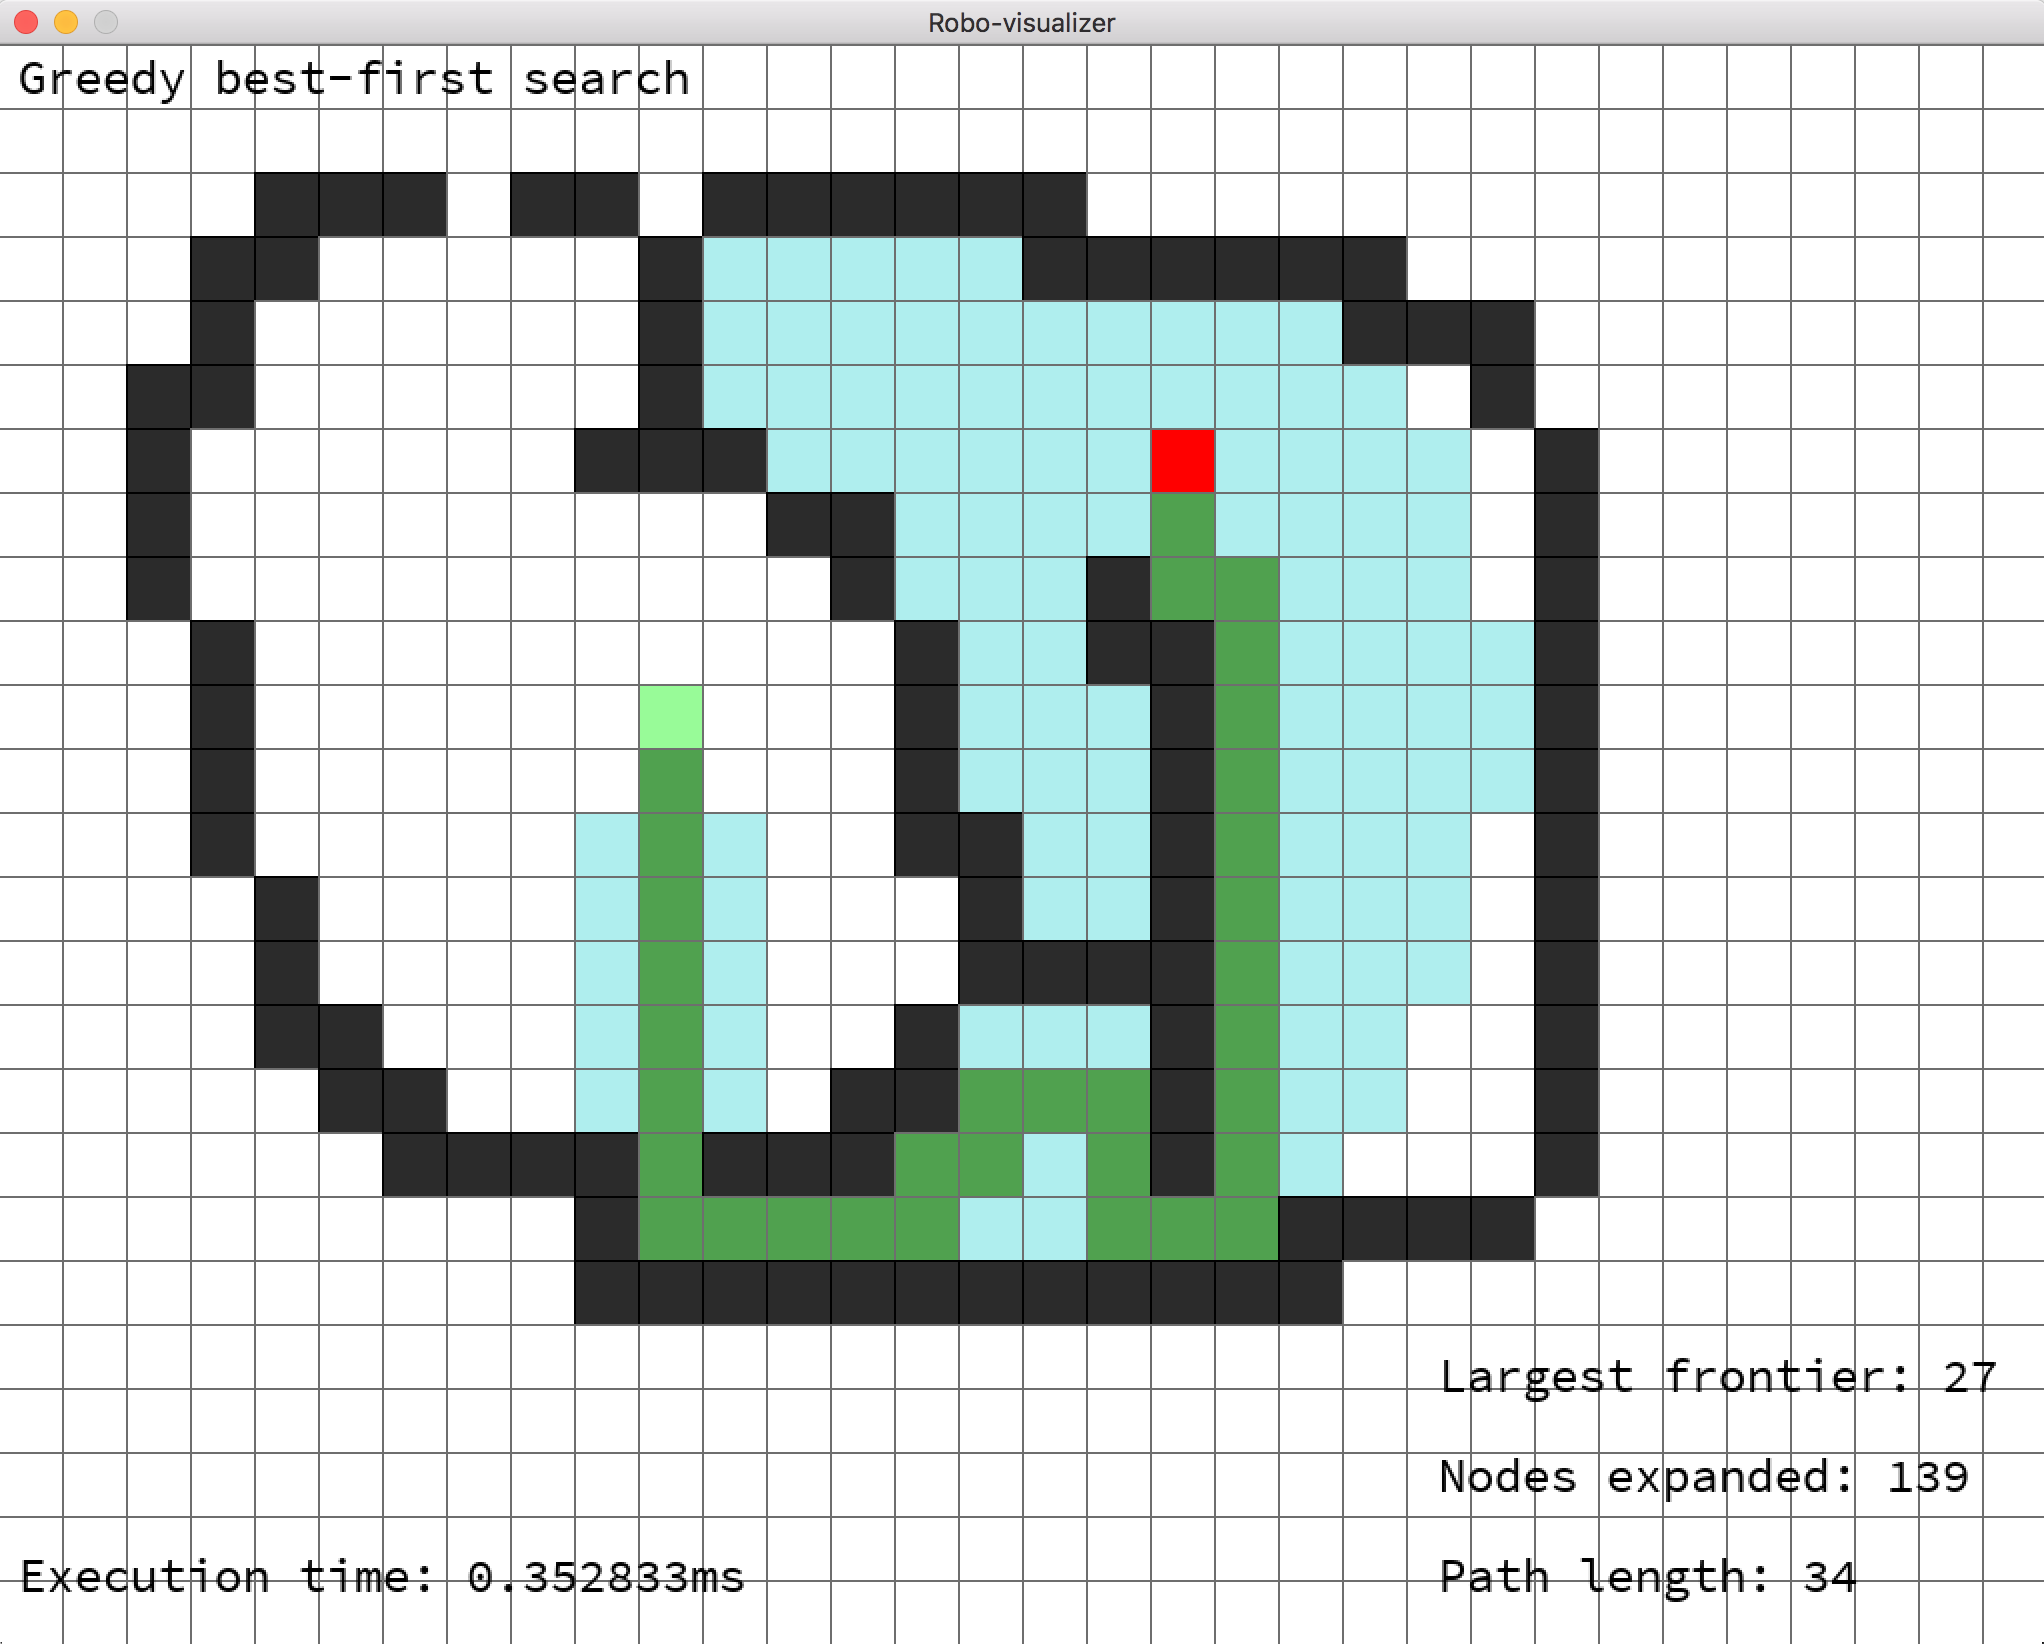
\includegraphics[width=0.6\textwidth]{Resources/vis.png}
	\caption{Screenshot of the GUI pathfinding visualizer}
\end{figure}

% subsection visualizer (end)

\subsection{Search Method Analysis} % (fold)
\label{sub:search_method_analysis}
While each search method has been discussed at a high level, this section aims to find the most effective search algorithm for the RNP. A method for random-generation of search problems with expected optimal paths was developed for the purpose of testing each search method across a variety of environments, with their time and memory usage recorded alongside the optimality of each solution.

\subsubsection{Methodology} % (fold)
\label{sub:methodology}

100 randomly generated search spaces were generated for grids of sizes $16 \times 16$, $32 \times 32$, and $64 \times 64$, 300 samples in total. Each search method was made to solve the sample recording their average run-time, number of nodes expanded, and other data of interest. Run-time and nodes expanded were chosen as data points for analysis as they demonstrate the time and space complexity of each search method, while path length was chosen to demonstrate optimality.

\paragraph{Search space generation} % (fold)
\label{par:search_space_generation}
Each cell in a grid was iterated over in a random order, with walls having a 15\% chance of being placed in each cell. Starting and ending positions were placed randomly, ensuring that no cells collided. As A* has been demonstrated to be both \textit{optimal} and \textit{complete}, with the implementations correctness having been proven through static tests as outlined in  on several pathfinding benchmarks, A* was used to calculate the optimal path as a benchmark for all subsequent tests.
% paragraph search_space_generation (end)

% subsubsection methodology (end)

\subsubsection{Results} % (fold)
\label{sub:results}
As outlined in table~\ref{tab:runtime_avgs}, A* and Greedy Best-First had the lowest mean run-times ($\mu=10.65$, $\mu=9.78$ respectively), while both iterative deepening methods had the highest. Furthermore the higher run-times had the highest standard deviations ($\sigma=142.93$ and $\sigma=6.22$).
% subsubsection results (end)

\begin{table}[H]
	\centering
	\input{Resources/Stats/table1}
	\caption{Averages and standard deviation for the run-time of each search method on all grids}
	\label{tab:runtime_avgs}
\end{table}

Table~\ref{tab:space_avgs} describes the average memory usage for each method, where GBFS and IDA* expanded the lowest number of nodes on average ($\mu=114.76$ and $\mu=511.21$), while IDDFS expanded the highest number ($\mu=19493.45$), with the highest standard deviation ($\sigma=36364.81$).

\begin{table}[H]
	\centering
	\input{Resources/Stats/table2}
	\caption{Averages and standard deviation for the amount of nodes expanded for each search method on all grids}
	\label{tab:space_avgs}
\end{table}

Figure~\ref{fig:idas_iddfs_runtime_dist} shows the distribution of run-times for different grid sizes for both IDA* and IDDFS, demonstrating the locations of outliers for each method.

\begin{figure}[H]
	\hfill
	\subfigure[IDA*]{\includegraphics[width=0.45\textwidth]{Resources/Stats/size_relationship_idas.pdf}}
	\hfill
	\subfigure[IDDFS]{\includegraphics[width=0.45\textwidth]{Resources/Stats/size_relationship_iddfs.pdf}}
	\caption{Distribution of run-times for each grid size for both IDA* and IDDFS}
	\label{fig:idas_iddfs_runtime_dist}
\end{figure}

Each search method had the same average path length ($\mu=27.94$), aside from GBFS which was slightly higher ($\mu=30.05$). DFS is excluded from the results here as its average path length ($\mu=372.64$) was, as expected, too large of an outlier to be of much use for comparisons. Figure~\ref{fig:expanded_walls_relationship} shows the linear relationship between the number of walls present in a grid and the number of nodes expanded per search. Both IDA* and IDDF are excluded from these results as neither method showed a significant relationship between these variables. Finally, while the number of solutions was recorded for each search method, the mean number of solutions found was the same for all methods ($\mu=92.47$).

\begin{figure}[H]
	\centering
	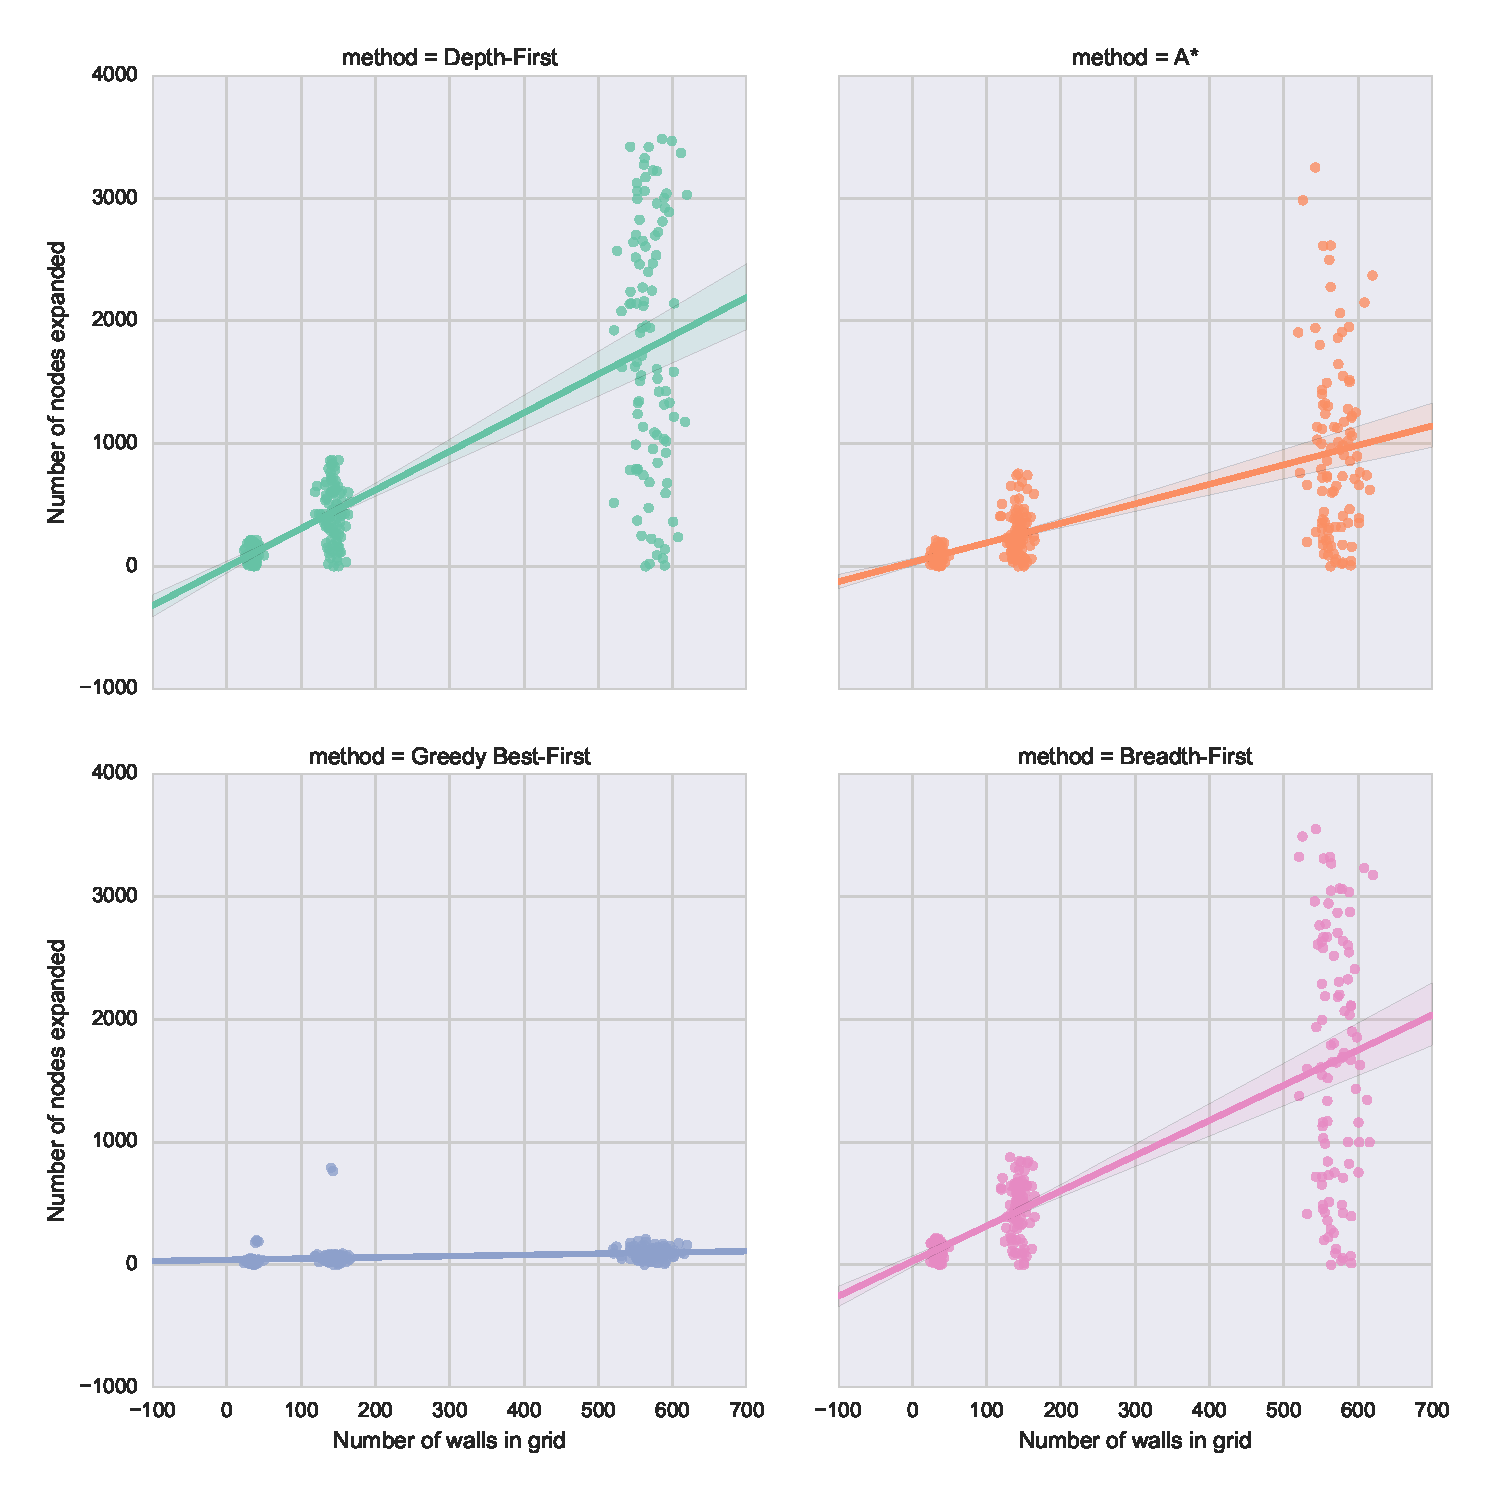
\includegraphics[width=0.65\textwidth]{Resources/Stats/walls_nodes_relationship.pdf}
	\caption{Linear relationship between number of walls in a grid and the number of nodes expanded}
	\label{fig:expanded_walls_relationship}
\end{figure}

\subsubsection{Discussion} % (fold)
\label{sub:discussion}
As expected (discussed in section~\ref{sec:search_algorithms}) each search method excluding DFS and GBFS proved \textit{optimal} in all problems in which a solution existed. GBFS, while certainly non-optimal, had an average path length that proved not much longer than the optimal one with a lower standard deviation and proved to find solutions faster while expanding far fewer nodes than any other method, which indicates that although it may not always find the optimal solution for the RNP, it finds a \textit{good-enough} solution reliably while using much less resources in doing so - possibly suited for problems where some kind of kind of path, not necessarily the optimal one, is required in a short period of time.
\par
Of the \textbf{optimal} search methods, A* proved to have the most reliably efficient run-time whilst still remaining modest in terms of memory usage, demonstrating its usefulness as a general purpose search algorithm. Of note, is that IDA* expanded less nodes on average while still maintaining a modest run-time, this could be of use for computing environments with limited memory, however for environments where memory is plentiful the trade off in run-time may be too great to make IDA* worth utilizing. Finally, of the custom and iterative methods, IDDFS proved to be an outlier with both the amount of nodes expanded and its average run-time proved quite high. However, as highlighted in figure~\ref{fig:idas_iddfs_runtime_dist}, IDDFS showed a few very high outliers for larger grids with the distribution of run-times existing at the lower end for other grid sizes, which may indicate that while IDDFS is certainly optimal and can be efficient it may prove too unreliable to be of use for problems such as the RNP.
% subsubsection discussion (end)

% subsection search_method_analysis (end)

% section research (end)
